% !TEX program = xelatex
% Supplementary Information (English only)
% Compile: xelatex supplementary_information_en.tex
\documentclass[11pt,a4paper]{article}

\usepackage[margin=2.4cm]{geometry}
\usepackage{amsmath,amssymb}
\usepackage{graphicx}
\usepackage{setspace}
\usepackage{parskip}
\usepackage{titlesec}
\usepackage{booktabs}
\usepackage{tabularx}
\usepackage{multirow}
\usepackage{hyperref}
\usepackage{xcolor}
\usepackage{caption}
\usepackage{longtable}
\usepackage{array}
\usepackage{fontspec}

\setmainfont{Times New Roman}

\titleformat{\section}{\normalfont\large\bfseries}{\thesection}{0.6em}{}
\titleformat{\subsection}{\normalfont\normalsize\bfseries}{\thesubsection}{0.5em}{}

\setlength{\parskip}{0.6em}
\setlength{\parindent}{0pt}
\onehalfspacing

% Figure path
\graphicspath{{../../0414_v4/figures/}}

% Convenience macros
\newcommand{\keff}{\ensuremath{k_{\mathrm{eff}}}}
\newcommand{\Eint}{\ensuremath{E_{\mathrm{intercept}}}}
\newcommand{\Eslope}{\ensuremath{E_{\mathrm{slope}}}}
\newcommand{\abase}{\ensuremath{\alpha_{\mathrm{base}}}}
\newcommand{\aslope}{\ensuremath{\alpha_{\mathrm{slope}}}}
\newcommand{\kref}{\ensuremath{k_{\mathrm{ref}}}}
\newcommand{\Tref}{\ensuremath{T_{\mathrm{ref}}}}
\newcommand{\kslope}{\ensuremath{k_{\mathrm{slope}}}}

\title{\textbf{Supplementary Information}\\[0.3em]
\large Bayesian Neural Surrogates Unify Uncertainty Propagation,\\
Sensitivity Attribution and Calibration for Coupled\\
Multi-Physics Reactor Analysis}
\author{Yinuo Chen, Sicheng Wang, Xiaojing Liu*, Tengfei Zhang*}
\date{}

\begin{document}
\maketitle

\tableofcontents
\newpage

% ======================================================================
\section{Supplementary Figures}
\label{sec:figures}
% ======================================================================

% --- Fig. S1 ---
\begin{figure}[htbp]
\centering

\includegraphics[width=\textwidth]{fig0_workflow.pdf}
\caption{\textbf{Fig.~S1~|~BNN surrogate workflow.}
Schematic of the end-to-end probabilistic analysis framework. The BNN
surrogate is trained on coupled OpenMC--FEniCS data and produces a
posterior predictive distribution. This single distribution serves as
the shared probabilistic layer for forward uncertainty propagation,
Sobol sensitivity attribution, and MCMC posterior calibration, without
retraining between analyses.}
\label{fig:S1}
\end{figure}

% --- Fig. S2 ---
\begin{figure}[htbp]
\centering

\includegraphics[width=\textwidth]{figA1_model_validation.pdf}
\caption{\textbf{Fig.~S2~|~Model validation: parity and residual analysis.}
Predicted versus true values and residual distributions for primary
outputs across both BNN variants (501 test samples). Shaded regions
show the 90\% predictive interval.}
\label{fig:S2}
\end{figure}

% --- Fig. S3 ---
\begin{figure}[htbp]
\centering
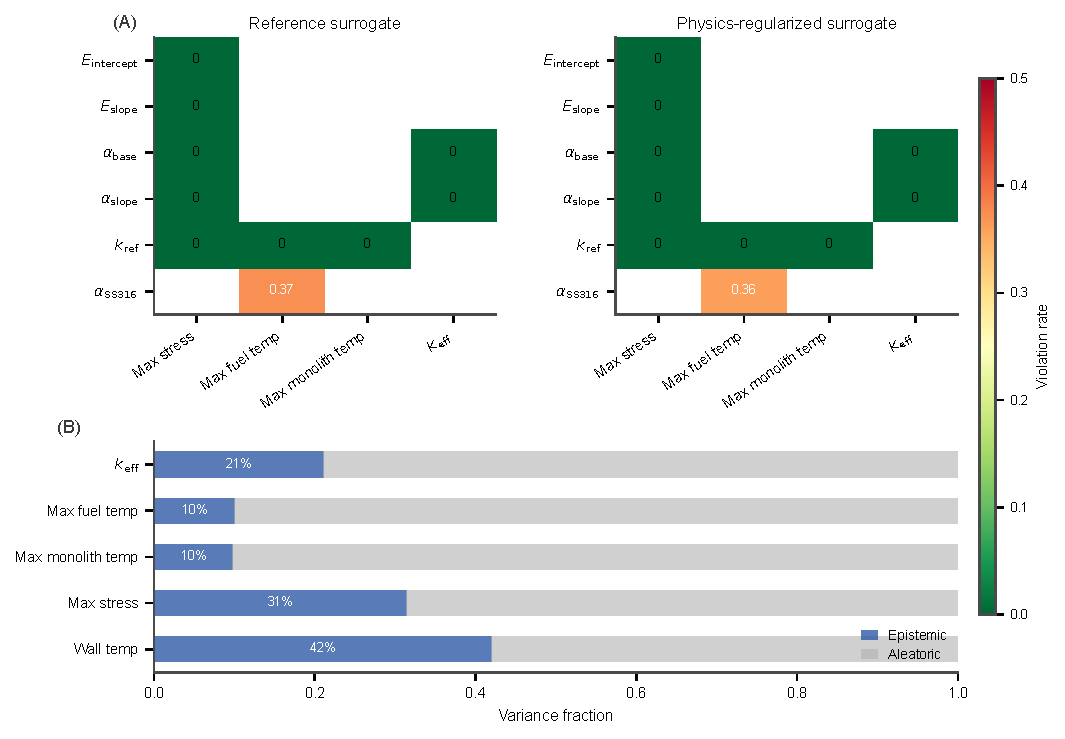
\includegraphics[width=\textwidth]{figA2_physics_robustness.pdf}
\caption{\textbf{Fig.~S3~|~Physics consistency and uncertainty decomposition.}
(\textbf{A})~Monotonicity violation rates for 15 input--output pairs
across both BNN variants; high-confidence pairs achieve zero violations.
(\textbf{B})~Epistemic vs.\ aleatoric variance decomposition. Aleatoric
uncertainty dominates across all outputs (58--90\% of total variance).}
\label{fig:S3}
\end{figure}

% --- Fig. S4 ---
\begin{figure}[htbp]
\centering

\includegraphics[width=\textwidth]{figS4_ood.pdf}
\caption{\textbf{Fig.~S4~|~Out-of-distribution (OOD) coverage and
epistemic uncertainty.}
90\% predictive interval coverage for in-distribution versus four
feature-tail subsets. Stress retains coverage above 0.75 across all
tails. \keff{} coverage degrades substantially on the \abase{} tail
($R^2$ drops to approximately 0.29), indicating that the Sobol and
posterior conclusions for \keff{} are valid only within the training
range of this dominant parameter. Elevated epistemic ratios on the
\abase{} tail confirm that the BNN correctly signals increased model
uncertainty outside the training domain.}
\label{fig:S4}
\end{figure}

% --- Fig. S5 ---
\begin{figure}[htbp]
\centering

\includegraphics[width=\textwidth]{figS1_sobol_convergence.pdf}
\caption{\textbf{Fig.~S5~|~Sobol index convergence with sample size.}
First-order Sobol index $S_1$ as a function of sample size $N_S$
(256 to 4096) for stress and \keff{}, with 90\% CI bands across
50 replications. Indices stabilise by $N_S = 2048$, confirming
convergence at the chosen $N_S = 4096$.}
\label{fig:S5}
\end{figure}

% --- Fig. S6 ---
\begin{figure}[htbp]
\centering
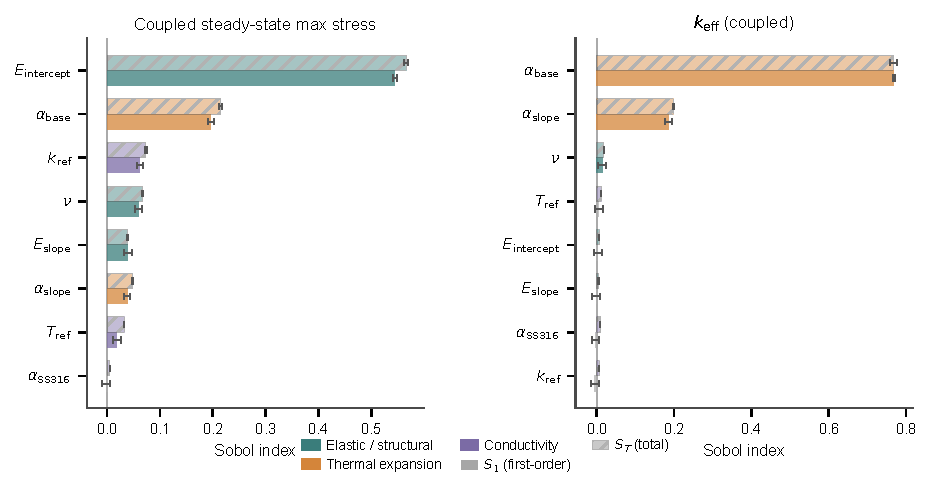
\includegraphics[width=\textwidth]{figA4_sobol_detail.pdf}
\caption{\textbf{Fig.~S6~|~Detailed Sobol sensitivity analysis.}
First-order and total-order Sobol indices for all eight material
parameters across all five primary outputs, showing the dominance
of \Eint{} for stress and \abase{} for \keff{}.}
\label{fig:S6}
\end{figure}

% --- Fig. S7 ---
\begin{figure}[htbp]
\centering

\includegraphics[width=\textwidth]{figS2_prior_sensitivity.pdf}
\caption{\textbf{Fig.~S7~|~Prior sensitivity analysis.}
Posterior marginal distributions for the four calibrated parameters
under six prior configurations: canonical, diffuse ($2\times$), tight
($0.5\times$), flat (uniform), shift$_{+}$ ($\mu + 0.5\sigma$),
shift$_{-}$ ($\mu - 0.5\sigma$). The tight prior over-constrains the
posterior, reducing coverage to 50--83\% (Table~S10).}
\label{fig:S7}
\end{figure}

% --- Fig. S8 ---
\begin{figure}[htbp]
\centering
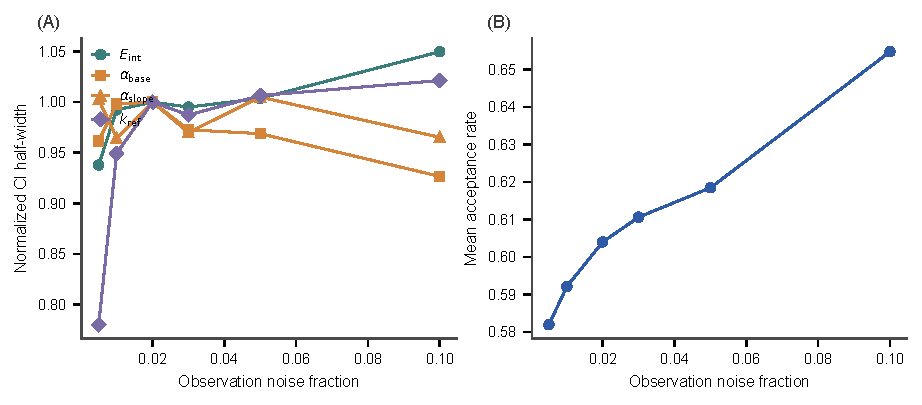
\includegraphics[width=\textwidth]{figS3_noise_sensitivity.pdf}
\caption{\textbf{Fig.~S8~|~Observation noise sensitivity.}
Posterior width and acceptance rate as a function of assumed observation
noise fraction (0.5\%--10\%). Posterior standard deviations increase
monotonically; acceptance rates increase appropriately as the likelihood
broadens (Table~S11).}
\label{fig:S8}
\end{figure}

% --- Fig. S9 ---
\begin{figure}[htbp]
\centering
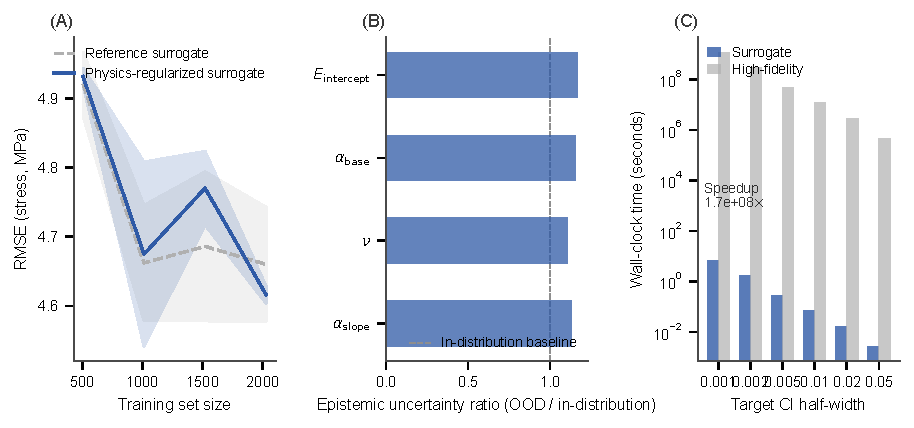
\includegraphics[width=\textwidth]{figA3_efficiency.pdf}
\caption{\textbf{Fig.~S9~|~Data efficiency and computational cost.}
Test RMSE and $R^2$ as a function of training set size for the
physics-regularized BNN. Near-saturated performance is achieved at
25\% data utilisation (507 training samples; Table~S12).}
\label{fig:S9}
\end{figure}

% --- Fig. S10 ---
\begin{figure}[htbp]
\centering
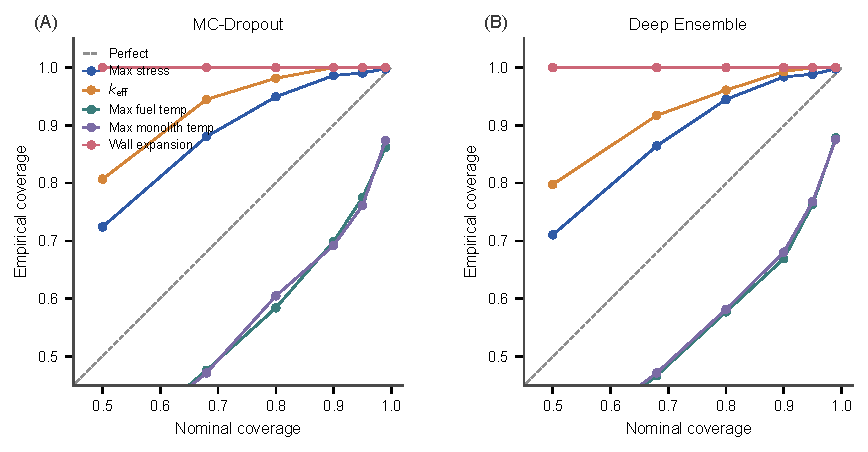
\includegraphics[width=\textwidth]{figS5_external_calib.pdf}
\caption{\textbf{Fig.~S10~|~External baseline calibration comparison.}
Calibration curves comparing BNN, MC-Dropout and deep ensemble across
primary outputs. The BNN achieves substantially better probabilistic
calibration (ECE 0.027 vs.\ 0.18--0.19) on temperature outputs.}
\label{fig:S10}
\end{figure}

\clearpage

% ======================================================================
\section{Supplementary Tables}
\label{sec:tables}
% ======================================================================

% --- Table S1 ---
\begin{table}[htbp]
\centering
\caption{\textbf{Table~S1~|~Material parameters: definitions, nominal values
and priors.}}
\label{tab:S1}
\smallskip
\small
\begin{tabular}{lllll}
\toprule
Parameter & Symbol & Nominal value & Unit & Prior range ($\pm$10\%) \\
\midrule
Young's mod.\ intercept & \Eint{} & $2\times10^{11}$ & Pa
  & $[1.8, 2.2]\times10^{11}$ \\
Young's mod.\ slope & \Eslope{} & $-7\times10^{7}$ & Pa/K
  & $[-7.7, -6.3]\times10^{7}$ \\
Poisson's ratio & $\nu$ & 0.31 & ---
  & [0.279, 0.341] \\
CTE base & \abase{} & $1\times10^{-5}$ & K$^{-1}$
  & $[0.9, 1.1]\times10^{-5}$ \\
CTE slope & \aslope{} & $5\times10^{-9}$ & K$^{-2}$
  & $[4.5, 5.5]\times10^{-9}$ \\
Ref.\ conductivity & \kref{} & 23.2 & W/(m$\cdot$K)
  & [20.88, 25.52] \\
Ref.\ temperature & \Tref{} & 923.15 & K
  & [830.84, 1015.47] \\
Cond.\ slope & \kslope{} & 1/75 & W/(m$\cdot$K$^2$)
  & [0.012, 0.0147] \\
\bottomrule
\end{tabular}
\end{table}

% --- Table S2 ---
\begin{table}[htbp]
\centering
\caption{\textbf{Table~S2~|~BNN hyperparameter search space and optimal
values.}}
\label{tab:S2}
\smallskip
\small
\begin{tabular}{lll}
\toprule
Hyperparameter & Search range & Optimal (bnn-phy-mono) \\
\midrule
Width           & [64, 256]           & 254 \\
Depth           & [2, 8]              & 2 \\
Learning rate   & [$10^{-4}$, $10^{-2}$] & $9.81\times10^{-4}$ \\
Weight decay    & [$10^{-9}$, $10^{-5}$] & $8.09\times10^{-8}$ \\
Batch size      & \{16, 32, 64\}      & 32 \\
Epochs          & [200, 500]          & 399 \\
Gradient clip   & [0.1, 2.0]          & 0.674 \\
$w_\mathrm{data}$ & [0.1, 5.0]       & 1.855 \\
Prior $\sigma$  & [0.1, 2.0]          & 0.478 \\
KL weight       & [$10^{-5}$, $10^{-2}$] & $1.93\times10^{-4}$ \\
$w_\mathrm{mono}$ & [0.01, 1.0]      & 0.212 \\
$\rho_\mathrm{abs,min}$ & [0.01, 0.5] & 0.123 \\
mono\_topk      & [10, 100]           & 53 \\
\bottomrule
\end{tabular}

\smallskip
Search: Optuna with 30 trials; objective: validation RMSE.
Activation: SiLU throughout. Output heads: mean + log-variance
(heteroscedastic).
\end{table}

% --- Table S3 ---
\begin{table}[htbp]
\centering
\caption{\textbf{Table~S3~|~BNN ablation study: reference baseline vs.\
physics-regularized surrogate} (mean $\pm$ s.d., 5 seeds).
Additional ablations (heteroscedastic noise, multi-fidelity architecture)
are in Notes~G--I.}
\label{tab:S3}
\smallskip
\small
\begin{tabular}{lccc}
\toprule
Model variant & Stress $R^2$ & Stress PICP & \keff{} $R^2$ \\
\midrule
Reference (ELBO only) & $0.936\pm0.007$ & $0.995\pm0.002$ & $0.633\pm0.260$ \\
Physics-regularized   & $0.935\pm0.007$ & $0.987\pm0.007$ & $0.633\pm0.258$ \\
\bottomrule
\end{tabular}
\end{table}

% --- Table S4 ---
\begin{table}[htbp]
\centering
\caption{\textbf{Table~S4~|~Complete Sobol indices ($S_1$ and $S_T$) for
stress and \keff{}} (physics-regularized BNN, $N_S = 4096$,
50 replications, 90\% CI).}
\label{tab:S4}
\smallskip
\small
\begin{tabular}{lcc}
\toprule
Parameter & Stress $S_1$ [90\% CI] & Stress $S_T$ [90\% CI] \\
\midrule
\Eslope{}    & 0.037 [$-$0.046, 0.100] & 0.039 [0.038, 0.039] \\
\Eint{}      & 0.548 [0.498, 0.572]    & 0.566 [0.562, 0.571] \\
$\nu$        & 0.063 [0.034, 0.097]    & 0.068 [0.067, 0.069] \\
\abase{}     & 0.210 [0.171, 0.254]    & 0.214 [0.212, 0.217] \\
\aslope{}    & 0.038 [$-$0.013, 0.091] & 0.047 [0.046, 0.049] \\
\Tref{}      & 0.019 [$-$0.025, 0.055] & 0.032 [0.031, 0.033] \\
\kref{}      & 0.065 [0.014, 0.118]    & 0.073 [0.072, 0.075] \\
SS316\_$\alpha$ & $-$0.004 [$-$0.068, 0.034] & 0.005 [0.005, 0.006] \\
\midrule
Parameter & \keff{} $S_1$ [90\% CI] & \keff{} $S_T$ [90\% CI] \\
\midrule
\Eslope{}    & 0.010 [$-$0.052, 0.062] & 0.005 [0.004, 0.005] \\
\Eint{}      & 0.008 [$-$0.065, 0.071] & 0.006 [0.006, 0.007] \\
$\nu$        & 0.029 [$-$0.035, 0.086] & 0.018 [0.018, 0.019] \\
\abase{}     & 0.771 [0.747, 0.788]    & 0.767 [0.758, 0.776] \\
\aslope{}    & 0.195 [0.112, 0.250]    & 0.198 [0.196, 0.201] \\
\Tref{}      & 0.010 [$-$0.023, 0.054] & 0.011 [0.011, 0.012] \\
\kref{}      & 0.000 [$-$0.063, 0.048] & 0.006 [0.006, 0.007] \\
SS316\_$\alpha$ & 0.003 [$-$0.059, 0.074] & 0.009 [0.009, 0.009] \\
\bottomrule
\end{tabular}
\end{table}

% --- Table S5 ---
\begin{table}[htbp]
\centering
\caption{\textbf{Table~S5~|~Posterior calibration: 18 benchmark case
summary} (physics-regularized BNN).}
\label{tab:S5}
\smallskip
\small
\begin{tabular}{clcccc}
\toprule
Case & Category & True stress (MPa) & Accept rate & 90\%-CI coverage & Post-mean err. \\
\midrule
 0 & low  & 110.3 & 0.607 & 3/4 &  8.3 \\
 1 & low  & 117.7 & 0.605 & 4/4 & 24.6 \\
 2 & low  &  98.7 & 0.632 & 1/4 &  9.0 \\
 3 & low  & 115.9 & 0.623 & 3/4 &  8.8 \\
 4 & low  &  96.8 & 0.612 & 2/4 &  3.1 \\
 5 & low  & 102.0 & 0.617 & 3/4 & 23.4 \\
 6 & near & 124.5 & 0.609 & 4/4 & 20.3 \\
 7 & near & 121.4 & 0.592 & 4/4 & 26.6 \\
 8 & near & 127.2 & 0.616 & 4/4 &  5.9 \\
 9 & near & 129.4 & 0.602 & 4/4 &  3.5 \\
10 & near & 122.4 & 0.597 & 4/4 &  4.5 \\
11 & near & 130.2 & 0.595 & 4/4 &  3.8 \\
12 & high & 135.0 & 0.608 & 4/4 &  0.2 \\
13 & high & 148.5 & 0.594 & 2/4 & 12.1 \\
14 & high & 141.2 & 0.582 & 4/4 & 13.7 \\
15 & high & 198.4 & 0.595 & 4/4 &  3.6 \\
16 & high & 133.2 & 0.622 & 4/4 & 10.5 \\
17 & high & 188.6 & 0.593 & 4/4 &  5.4 \\
\midrule
\multicolumn{2}{l}{Overall} & & 0.58--0.63 & 62/72 = 0.861 & MAE = 10.4 \\
\bottomrule
\end{tabular}
\end{table}

% --- Table S6 ---
\begin{table}[htbp]
\centering
\caption{\textbf{Table~S6~|~Computational cost breakdown.}}
\label{tab:S6}
\smallskip
\small
\begin{tabular}{lll}
\toprule
Operation & Time & Platform \\
\midrule
Coupled HF solve (1 case) & 2266\,s & EPYC 9654 / 96 cores \\
BNN single draw ($M=50$) & $1.29\times10^{-2}$\,s & GPU \\
BNN batched (batch=1024, per sample) & $1.34\times10^{-5}$\,s & GPU \\
20,000-sample forward UQ & ${\sim}0.3$\,s & GPU \\
Sobol (50 reps $\times$ 40,960 evals) & ${\sim}$minutes & GPU \\
18-case MCMC (8000 iter $\times$ 4 chains) & ${\sim}$minutes & GPU \\
\midrule
Speedup (single draw vs.\ HF) & $1.43\times10^{5}$ & \\
Speedup (batched vs.\ HF) & $1.37\times10^{8}$ & \\
\bottomrule
\end{tabular}
\end{table}

% --- Table S7 ---
\begin{table}[htbp]
\centering
\caption{\textbf{Table~S7~|~Physics consistency: monotonicity violation
rates} (501 test samples, discrete $\pm\delta$ perturbation test).}
\label{tab:S7}
\smallskip
\small
\begin{tabular}{lcc}
\toprule
Physics pair (input $\to$ output, sign) & Ref.\ BNN & Phy-reg \\
\midrule
\Eint{} $\to$ Max stress (+)     & 0\% & 0\% \\
\abase{} $\to$ Max stress (+)    & 0\% & 0\% \\
\abase{} $\to$ \keff{} ($-$)     & 0\% & 0\% \\
\kref{} $\to$ Max stress ($-$)   & 0\% & 0\% \\
SS316\_$\alpha$ $\to$ Fuel temp ($-$) & 36.3\% & 35.6\% \\
\bottomrule
\end{tabular}

\smallskip
Ordering/non-negativity constraints (max $\geq$ average temp, stress $\geq 0$):
0\% violations for both BNN variants.
\end{table}

% --- Table S8 ---
\begin{table}[htbp]
\centering
\caption{\textbf{Table~S8~|~Epistemic vs.\ aleatoric uncertainty
decomposition on test set.}}
\label{tab:S8}
\smallskip
\small
\begin{tabular}{lcccc}
\toprule
 & \multicolumn{2}{c}{Ref.\ BNN} & \multicolumn{2}{c}{Phy-reg BNN} \\
Output & Epi\% & Ale\% & Epi\% & Ale\% \\
\midrule
\keff{}            & 12.0 & 88.0 & 10.2 & 89.8 \\
Max fuel temp      & 12.0 & 88.0 & 10.1 & 89.9 \\
Max monolith temp  & 11.2 & 88.8 & 10.1 & 89.9 \\
Max stress         & 27.7 & 72.3 & 29.6 & 70.4 \\
Wall expansion     & 34.1 & 65.9 & 41.7 & 58.3 \\
\bottomrule
\end{tabular}
\end{table}

% --- Table S9 ---
\begin{table}[htbp]
\centering
\caption{\textbf{Table~S9~|~External baseline: full comparison of scoring
rules.}}
\label{tab:S9}
\smallskip
\small
\begin{tabular}{llccccc}
\toprule
Model & Output & RMSE & $R^2$ & CRPS & NLL & ECE \\
\midrule
MC-Dropout & \keff{} & 0.0003 & 0.856 & 0.0002 & $-$6.502 & 0.152 \\
           & Fuel temp   & 4.497 & 0.590 & 2.624 & 3.352 & 0.183 \\
           & Monolith T  & 5.061 & 0.590 & 2.951 & 3.472 & 0.182 \\
           & Max stress  & 7.659 & 0.934 & 4.519 & 3.592 & 0.118 \\
           & Wall exp.   & 0.0008 & 0.999 & 0.002 & $-$3.831 & 0.197 \\
\midrule
Deep Ensemble & \keff{} & 0.0003 & 0.828 & 0.0002 & $-$6.476 & 0.142 \\
              & Fuel temp   & 4.495 & 0.590 & 2.634 & 3.326 & 0.190 \\
              & Monolith T  & 5.061 & 0.590 & 2.962 & 3.439 & 0.185 \\
              & Max stress  & 7.644 & 0.934 & 4.502 & 3.586 & 0.112 \\
              & Wall exp.   & 0.0006 & 0.999 & 0.002 & $-$3.841 & 0.197 \\
\bottomrule
\end{tabular}
\end{table}

% --- Table S10 ---
\begin{table}[htbp]
\centering
\caption{\textbf{Table~S10~|~Prior sensitivity} (6 configurations,
physics-regularized BNN, case 06, near-threshold).}
\label{tab:S10}
\smallskip
\small
\begin{tabular}{lccc}
\toprule
Prior variant & Coverage (4 params) & Mean KL vs.\ canonical & Accept rate \\
\midrule
Canonical         & 100\%      & 0.00 (reference) & 0.61 \\
Diffuse ($2\times$)  & 100\%   & 0.15--0.22       & 0.63 \\
Tight ($0.5\times$)  & 50--83\% & 0.64--1.28      & 0.57 \\
Flat (uniform)    & 100\%      & 0.24--0.38       & 0.64 \\
Shift ($+0.5\sigma$) & 67--100\% & 0.06--0.36    & 0.60 \\
Shift ($-0.5\sigma$) & 83--100\% & 0.08--0.28    & 0.61 \\
\bottomrule
\end{tabular}
\end{table}

% --- Table S11 ---
\begin{table}[htbp]
\centering
\caption{\textbf{Table~S11~|~Noise sensitivity} (noise fraction
0.5\%--10\%, physics-regularized BNN, case 06).}
\label{tab:S11}
\smallskip
\small
\begin{tabular}{lccc}
\toprule
Noise fraction & \Eint{} post.\ std & Accept rate & Coverage \\
\midrule
0.5\%            & $1.26\times10^{10}$ & 0.58 & 100\% \\
1.0\%            & $1.28\times10^{10}$ & 0.59 & 100\% \\
2.0\% (default)  & $1.32\times10^{10}$ & 0.61 & 100\% \\
5.0\%            & $1.36\times10^{10}$ & 0.63 & 100\% \\
10.0\%           & $1.40\times10^{10}$ & 0.65 &  83\% \\
\bottomrule
\end{tabular}
\end{table}

% Table S12 (data efficiency) superseded by Note G (Table S13)
% with v3418 dataset results. See Section~\ref{sec:noteG}.

\clearpage

% ======================================================================
\section{Supplementary Notes}
\label{sec:notes}
% ======================================================================

\subsection{Note A: BNN training details}

\subsubsection*{A.1.~Evidence lower bound (ELBO) derivation}

The BNN posterior over weights $\mathbf{w}$ is approximated by a
mean-field variational distribution
$q(\mathbf{w}) = \prod_i \mathcal{N}(w_i \mid \mu_i, \sigma_i^2)$.
The variational parameters are optimised by minimising the negative
evidence lower bound:
\begin{equation}
\mathcal{L}(\boldsymbol{\mu}, \boldsymbol{\sigma})
= \mathrm{KL}\bigl[q(\mathbf{w}) \,\|\, p(\mathbf{w})\bigr]
- \mathbb{E}_{q(\mathbf{w})}\bigl[\log p(\mathcal{D} \mid \mathbf{w})\bigr]
\end{equation}
where $p(\mathbf{w}) = \mathcal{N}(\mathbf{0}, \sigma_p^2 \mathbf{I})$
is the isotropic Gaussian prior. The KL divergence admits a closed form;
the data-fit term is approximated by a single Monte Carlo sample per
mini-batch (Bayes-by-Backprop\textsuperscript{10}).

The reparameterisation trick enables gradient computation:
$w = \mu + \sigma \cdot \epsilon$, where
$\epsilon \sim \mathcal{N}(0, \mathbf{I})$. The variance parameter
$\sigma = \log(1 + \exp(\rho))$ ensures positivity, with
$\rho_\mathrm{abs,min}$ clamping $\rho \geq \rho_\mathrm{abs,min}$
to prevent posterior collapse.

\subsubsection*{A.2.~Heteroscedastic observation noise}

The network outputs both a mean $\mu(\boldsymbol{\theta})$ and a
log-variance $\log \sigma^2_\mathrm{obs}(\boldsymbol{\theta})$ per
output channel:
\begin{equation}
\log p(y_j \mid \boldsymbol{\theta}, \mathbf{w})
= -\tfrac{1}{2}\bigl[\log \sigma^2_{\mathrm{obs},j}
+ (y_j - \mu_j)^2 / \sigma^2_{\mathrm{obs},j}\bigr]
\end{equation}
This heteroscedastic formulation allows the BNN to model
input-dependent observation noise, separating it from epistemic
(weight) uncertainty.

\subsubsection*{A.3.~KL annealing schedule}

The KL weight $\beta$ is annealed from 0 to its target value
$\mathrm{kl\_weight} = 1.93\times10^{-4}$ over the first 100 epochs:
$\beta(t) = \min(t/100, 1) \cdot \mathrm{kl\_weight}$.
This prevents the KL term from dominating early training before the
data-fit term has found a reasonable region of weight space.

\subsubsection*{A.4.~Physics-prior monotonicity constraints}

The physics-regularized BNN adds an auxiliary loss:
\begin{equation}
\mathcal{L}_\mathrm{mono}
= \frac{1}{K}\sum_{k=1}^{K}\max\bigl(0,\;
  -\mathrm{sign}\cdot\partial\mu/\partial\theta_k\bigr)
\end{equation}
weighted by $w_\mathrm{mono} = 0.212$. Sign constraints are derived
from constitutive physics---for example, stress increases with \Eint{}
because $\sigma = \mathbf{C}(E, \nu) \cdot \boldsymbol{\epsilon}$ and
$\mathbf{C}$ is linear in $E$.

These are physics-prior constraints derived from constitutive
relationships.

\subsubsection*{A.5.~Gradient clipping and initialisation}

Gradient norms are clipped at 0.674 per parameter group. Weight means
$\mu$ are initialised with Xavier uniform; $\rho$ values are initialised
uniformly in $[-5, -4]$, corresponding to small initial variance. These
choices stabilise early training when the KL term is annealed in.


\subsection{Note B: Sobol sensitivity methodology}

\subsubsection*{B.1.~Sobol variance decomposition}

For a square-integrable function $f(\theta_1, \ldots, \theta_d)$ with
independent inputs, the total variance $V = \mathrm{Var}[f]$ can be
decomposed as:
\begin{equation}
V = \sum_i V_i + \sum_{i<j} V_{ij} + \cdots + V_{1,\ldots,d}
\end{equation}
The first-order Sobol index is $S_i = V_i / V$; the total-order index
is $S_{T,i} = 1 - V_{\sim i} / V$.

\subsubsection*{B.2.~Saltelli cross-matrix scheme}

Two independent $N \times d$ matrices $\mathbf{A}$ and $\mathbf{B}$ are
drawn from the joint prior. For each input $i$, a cross-matrix
$\mathbf{A}_\mathbf{B}^{(i)}$ is constructed by replacing the $i$-th
column of $\mathbf{A}$ with the $i$-th column of $\mathbf{B}$. The model
is evaluated at all $N(d+2)$ points.

\subsubsection*{B.3.~Jansen estimator}

\begin{align}
S_{1,i} &= 1 - \frac{1}{2N}\sum_{j=1}^{N}
  \bigl[f(\mathbf{A}_\mathbf{B}^{(i)})_j - f(\mathbf{B})_j\bigr]^2 / V \\
S_{T,i} &= \frac{1}{2N}\sum_{j=1}^{N}
  \bigl[f(\mathbf{A})_j - f(\mathbf{A}_\mathbf{B}^{(i)})_j\bigr]^2 / V
\end{align}
The Jansen estimator is preferred for its lower variance compared to
the Sobol estimator, particularly for indices near zero.

\subsubsection*{B.4.~Replication-based confidence intervals}

The entire Sobol analysis (sample generation, model evaluation, index
estimation) is independently repeated $R = 50$ times. The 90\%
confidence interval for each index is constructed from the 5th and 95th
percentiles of the $R$ replications. A factor is declared a stable
contributor only if the lower bound of its 90\% CI exceeds zero.

The BNN posterior predictive mean (averaged over $M = 30$ weight
samples) serves as the deterministic function $f(\boldsymbol{\theta})$
in the Sobol framework.


\subsection{Note C: MCMC posterior calibration details}

\subsubsection*{C.1.~Likelihood formulation}

\begin{equation}
\log p(\mathbf{y}_\mathrm{obs} \mid \boldsymbol{\theta})
= \sum_{j=1}^{J} \log \mathcal{N}\bigl(y_{\mathrm{obs},j} \mid
  \mu_j(\boldsymbol{\theta}),\;
  \sigma_{\mathrm{obs},j}^2 + \sigma_{\mathrm{BNN},j}^2(\boldsymbol{\theta})\bigr)
\end{equation}
where $\mu_j(\boldsymbol{\theta})$ is the BNN posterior predictive mean
(averaged over $M = 20$ weight samples),
$\sigma_{\mathrm{BNN},j}^2$ is the BNN aleatoric variance, and
$\sigma_{\mathrm{obs},j}^2$ is the observation noise variance (2\% of
the true value). The $J = 5$ primary outputs are: coupled peak global
stress, coupled peak fuel temperature, coupled peak monolith
temperature, coupled wall expansion, and \keff{}.

\subsubsection*{C.2.~Proposal distribution}

A symmetric Gaussian random-walk proposal is used:
$\boldsymbol{\theta}^* = \boldsymbol{\theta}_\mathrm{current} +
\boldsymbol{\epsilon}$,
$\boldsymbol{\epsilon} \sim \mathcal{N}(\mathbf{0},
\boldsymbol{\Sigma}_\mathrm{proposal})$,
where $\boldsymbol{\Sigma}_\mathrm{proposal} =
\mathrm{diag}(\mathrm{scale}_1^2, \ldots, \mathrm{scale}_4^2)$.
The proposal scales were calibrated by short pilot runs of 1000
iterations.

\subsubsection*{C.3.~Chain configuration}

For each benchmark case:
\begin{itemize}
\item 4 independent chains with dispersed initialisations drawn from
  the prior
\item $N_\mathrm{total} = 8000$ iterations per chain
\item Burn-in: first 2000 iterations discarded
\item Thinning: every 5th post-burn-in sample retained
\item Effective posterior: 1200 samples per chain, 4800 total per case
\end{itemize}

The four calibrated parameters are \Eint{}, \abase{}, \aslope{}, and
\kref{}, selected as the four with the largest Sobol total-order indices
across stress and \keff{}. The remaining four parameters (\Eslope{},
$\nu$, \Tref{}, \kslope{}) are fixed at their true values.

\subsubsection*{C.4.~Convergence diagnostics}

Convergence is assessed by:
\begin{enumerate}
\item Visual inspection of trace plots (Fig.~S9 in the main text
  references)
\item Rank-normalised split-$\hat{R}$ (Vehtari et al.\ 2021):
  $\hat{R}_\mathrm{max} = 1.017$ across all 72 parameter--case
  combinations, well below the 1.1 threshold
\item Geyer initial-positive-sequence effective sample size:
  $\mathrm{ESS}_\mathrm{min} = 352$ (all cases)
\item Acceptance rates: range 0.58--0.62, mean 0.605 (Table~S5)
\end{enumerate}

\subsubsection*{C.5.~Benchmark case selection}

The 18 benchmark cases are drawn from the 501-sample test split:
\begin{itemize}
\item 6 low-stress cases (true stress 102--119\,MPa)
\item 6 near-threshold cases (true stress 123--129\,MPa)
\item 6 high-stress cases (true stress 143--198\,MPa)
\end{itemize}
The threshold for categorisation is the primary safety threshold of
131\,MPa. For each case, the ``observation'' is the true HF output
vector perturbed by 2\% multiplicative Gaussian noise.


\subsection{Note D: Forward UQ extensions}

\subsubsection*{D.1.~Posterior predictive mean vs.\ full predictive draw}

The main-text forward UQ propagates through the BNN posterior predictive
mean $y = \mathbb{E}_{\mathbf{w}}[\mu_{\mathbf{w}}(\boldsymbol{\theta})]$,
isolating parametric uncertainty from the BNN's own epistemic and
aleatoric spread. As a consistency check, full predictive draws
(sampling both weight uncertainty and observation noise) produce wider
distributions but consistent means and percentile rankings, confirming
that the parametric sensitivity structure is robust to the choice of
predictive protocol.

\subsubsection*{D.2.~Latin hypercube sampling}

Latin hypercube sampling (LHS) is used rather than simple random
sampling because LHS ensures more uniform coverage of the input space,
reducing sampling variance for a given sample size. With $N = 20{,}000$
samples and $d = 8$ inputs, the LHS design partitions each input
dimension into 20,000 equal-probability intervals.


\subsection{Note E: Coupled simulation and material model details}

\subsubsection*{E.1.~Material constitutive models}

The SS316 monolith is the structural component that simultaneously
bears thermal stress and transmits heat between fuel and heat pipes.
All eight uncertain parameters enter the calculation through the
constitutive models:
\begin{itemize}
\item \textbf{Structural mechanics:}
  $E(T) = \Eslope{} \cdot T + \Eint{}$; $\nu$ (Poisson's ratio).
  Stress: $\sigma = \mathbf{C}(E, \nu) \cdot \boldsymbol{\epsilon}$.
\item \textbf{Thermal deformation:}
  $\alpha(T) = \abase{} + \aslope{} \cdot T$.
  Dual role: thermal strain
  $\epsilon_\mathrm{th} = \alpha \cdot \Delta T$ and geometric
  expansion.
\item \textbf{Thermal transport:}
  $k(T) = \kref{} + \kslope{} \cdot (T - \Tref{})$.
\end{itemize}

\subsubsection*{E.2.~Picard iteration and convergence}

The OpenMC--FEniCS coupling proceeds as:
\begin{enumerate}
\item Initialise with the eight material parameters and reference
  geometry.
\item OpenMC computes \keff{} and the spatially resolved fission power
  distribution.
\item FEniCS solves for the temperature field, thermal expansion
  displacement and stress field.
\item The updated geometry and temperature-dependent material
  cross-sections are fed back to OpenMC.
\item Steps 2--4 repeat until convergence.
\end{enumerate}
Convergence criterion: maximum temperature difference between
consecutive iterations $< 1$\,K. Under-relaxation factor: 0.1.

\subsubsection*{E.3.~Output definitions}

Each HF evaluation produces 15 scalar outputs: 7 decoupled (before
coupling convergence) and 8 coupled (after full convergence, including
\keff{}). The posterior likelihood uses 5 primary outputs: \keff{}, peak
fuel temperature, peak monolith temperature, peak global stress, and
wall expansion.

\subsubsection*{E.4.~Dataset generation}

$n = 3418$ samples were generated by Latin hypercube sampling over the
8-dimensional prior. The split (seed $= 2026$): training 2339 ($\sim$70\%),
validation 501 ($\sim$15\%), test 501 ($\sim$15\%). The fixed split is reused
across all experiments for reproducibility.


% ======================================================================
\subsection{Note F: High-fidelity coupled simulation framework}
\label{sec:noteF}
% ======================================================================

This note provides the governing equations of the four solver modules
that generate the coupled training data consumed by the BNN surrogate.
The framework couples OpenMC (neutron transport), FEniCS
(thermo-elasticity), a one-dimensional heat-pipe thermal--hydraulic
model and a fuel-temperature module via Picard fixed-point iteration.
Details follow the implementation described in Refs.~[9,~11].

% ------ F.1 ------
\subsubsection*{F.1.~Neutron transport --- OpenMC}

OpenMC~[11] is an open-source Monte Carlo particle transport code
supporting fixed-source, $k$-eigenvalue and subcritical multiplication
calculations. In the coupled framework it computes \keff{}, the
fission power distribution and auxiliary neutronic tallies.

\paragraph{Integral transport equation.}
The steady-state, continuous-energy neutron transport equation in
integral form reads
\begin{equation}
\Phi(\mathbf{r},\boldsymbol{\Omega},E)
= \int_{0}^{\infty}
  e^{-\tau(\mathbf{r},\mathbf{r}-s\boldsymbol{\Omega},E)}\,
  Q(\mathbf{r}-s\boldsymbol{\Omega},\boldsymbol{\Omega},E)\,\mathrm{d}s
\label{eq:integral_transport}
\end{equation}
where $\Phi$ is the angular neutron flux at position $\mathbf{r}$,
direction $\boldsymbol{\Omega}$ and energy $E$; $Q$ is the emission
density (scattering $+$ fission source); and $\tau$ is the optical
thickness:
\begin{equation}
\tau(\mathbf{r},\mathbf{r}',E)
= \int_{0}^{|\mathbf{r}-\mathbf{r}'|}
  \Sigma_t(\mathbf{r}-s\boldsymbol{\Omega},E)\,\mathrm{d}s
\end{equation}
with $\Sigma_t$ the macroscopic total cross-section.

\paragraph{Emission density and Fredholm formulation.}
Substituting the scattering and fission kernels into the emission
density yields the second-kind Fredholm integral equation:
\begin{equation}
Q(\mathbf{r},\boldsymbol{\Omega},E)
= \int K(\mathbf{r}',\boldsymbol{\Omega}',E'
        \to \mathbf{r},\boldsymbol{\Omega},E)\,
  Q(\mathbf{r}',\boldsymbol{\Omega}',E')\,
  \mathrm{d}\mathbf{r}'\,\mathrm{d}\boldsymbol{\Omega}'\,\mathrm{d}E'
\end{equation}
where the integral kernel $K$ is the product of a transport kernel
(free-flight attenuation) and a collision kernel (scattering $+$
fission). Writing this in operator form $Q = \mathcal{K}Q$ and
iterating:
\begin{equation}
Q^{(n+1)} = \mathcal{K}\,Q^{(n)},
\qquad
Q = \lim_{n\to\infty} Q^{(n)}
  = \sum_{k=0}^{\infty}\mathcal{K}^k\,Q^{(0)}
\end{equation}
which is the Neumann series solution. The converged $Q$ is substituted
back into Eq.~(\ref{eq:integral_transport}) to recover the full neutron
flux distribution.

\paragraph{Monte Carlo $k$-eigenvalue calculation.}
In practice, the integral equation is solved stochastically: a
population of $N_p$ neutron histories is tracked through successive
fission generations. Each generation produces an estimate of
\begin{equation}
k_{\mathrm{eff}}
= \frac{\text{neutron production in generation } n+1}
       {\text{neutron production in generation } n}
\end{equation}
and the converged fission source gives the spatial power distribution.
The statistical uncertainty on \keff{} is kept below 10\,pcm
($1\sigma$) and the maximum power-distribution standard deviation below
0.19\,\% by using a sufficiently large number of particle histories per
batch.

\paragraph{Geometry and temperature feedback.}
Thanks to the constructive solid geometry representation in OpenMC, the
framework updates fuel-rod and heat-pipe coordinates (reflecting
thermal expansion), material temperatures (Doppler broadening) and
material densities (thermal expansion) between coupling iterations.


% ------ F.2 ------
\subsubsection*{F.2.~Thermo-elastic analysis --- FEniCS}

The thermo-elastic module is built on the open-source finite-element
platform FEniCS~[12]. It solves two coupled problems on the monolith
mesh: steady-state heat conduction and linear thermoelasticity.

\paragraph{Heat conduction.}
The steady-state heat equation on the monolith domain $\Omega$ is
\begin{equation}
-\nabla\cdot\bigl[k(T)\,\nabla T\bigr] = \dot{q}
\qquad \text{in } \Omega
\label{eq:heat}
\end{equation}
where $k(T)$ is the temperature-dependent thermal conductivity of
SS316 (see Note~E) and $\dot{q}$ is the volumetric heat generation
rate from fission. Boundary conditions are: isothermal walls at heat-pipe
surfaces (temperatures from the heat-pipe module) and prescribed heat
fluxes at fuel-rod surfaces (from the power distribution).

\paragraph{Linear thermoelasticity.}
For an isotropic material, the three-dimensional linear elastic
constitutive relation (generalised Hooke's law) is
\begin{equation}
\boldsymbol{\sigma}
= \lambda\,\mathrm{tr}(\boldsymbol{\varepsilon})\,\mathbf{I}
  + 2\mu\,\boldsymbol{\varepsilon}
\label{eq:hooke}
\end{equation}
where $\boldsymbol{\sigma}$ is the Cauchy stress tensor,
$\boldsymbol{\varepsilon}$ the strain tensor, $\mathbf{I}$ the identity
tensor, and $\lambda,\mu$ are the Lam\'{e} constants determined by the
temperature-dependent Young's modulus $E(T)$ and Poisson's ratio $\nu$:
\begin{equation}
\lambda = \frac{E\,\nu}{(1+\nu)(1-2\nu)},
\qquad
\mu = \frac{E}{2(1+\nu)}
\label{eq:lame}
\end{equation}

\paragraph{Thermal strain (Duhamel--Neumann law).}
Including thermal deformation, the constitutive equation for an
isotropic solid becomes
\begin{equation}
\boldsymbol{\sigma}
= \lambda\,\mathrm{tr}(\boldsymbol{\varepsilon})\,\mathbf{I}
  + 2\mu\,\boldsymbol{\varepsilon}
  - (3\lambda + 2\mu)\,\alpha(T)\,\Delta T\,\mathbf{I}
\label{eq:duhamel}
\end{equation}
where $\alpha(T) = \abase{} + \aslope{}\cdot T$ is the
temperature-dependent coefficient of thermal expansion (CTE) and
$\Delta T = T - T_0$ is the temperature rise from the stress-free
reference state. The thermal strain tensor is
$\boldsymbol{\varepsilon}_{\mathrm{th}} = \alpha\,\Delta T\,\mathbf{I}$.

\paragraph{Equilibrium equation.}
The static momentum balance (in the absence of body forces other than
thermal loading) is
\begin{equation}
\nabla \cdot \boldsymbol{\sigma} = \mathbf{0}
\qquad \text{in } \Omega
\end{equation}
which, combined with Eqs.~(\ref{eq:duhamel}) and the strain--displacement
relation
$\boldsymbol{\varepsilon} = \tfrac{1}{2}(\nabla\mathbf{u} +
\nabla\mathbf{u}^T)$, yields the displacement field $\mathbf{u}$ and
the von~Mises stress $\sigma_\mathrm{vM}$ used as the primary stress
output.


% ------ F.3 ------
\subsubsection*{F.3.~Heat-pipe thermal--hydraulic model}

Each sodium heat pipe is modelled with one-dimensional transient
conservation equations for the vapour core and the porous wick. The
model captures evaporation, vapour transport, condensation and capillary
return, producing the steady-state wall temperature for a given input
power~[9].

\paragraph{Vapour continuity.}
\begin{equation}
\frac{\partial \rho_v}{\partial t}
+ \frac{\partial(\rho_v\,u_v)}{\partial z}
= \frac{\dot{m}_v}{D_v}
\end{equation}
where $\rho_v$, $u_v$ are the vapour density and axial velocity, $z$
the axial coordinate, $\dot{m}_v$ the mass source from evaporation and
$D_v$ the vapour-core diameter.

\paragraph{Liquid continuity in the wick.}
\begin{equation}
\frac{\partial(\phi\,S\,\rho_l)}{\partial t}
+ \frac{\partial(\phi\,S\,\rho_l\,u_l)}{\partial z}
= \frac{\dot{m}_l}{D_w}
\end{equation}
where $\phi$ is the wick porosity, $S$ the liquid fraction, $\rho_l$
and $u_l$ the liquid density and velocity, $\dot{m}_l$ the condensation
mass source.

\paragraph{Dusty-gas vapour transport.}
To handle the transition between free-molecular and continuum flow
regimes inside the vapour core, a second-order dusty-gas model~[13] is
employed:
\begin{equation}
\frac{\partial(\rho_v\,u_v)}{\partial z}
+ \frac{\partial}{\partial z}
  \Bigl(\rho_v\,u_v^2 + \rho_v\,R_g\,T\Bigr)
= -F_\mathrm{wall}
\end{equation}
where $R_g$ is the specific gas constant and $F_\mathrm{wall}$
represents the axial flow-diffusion coefficient including wall--molecule
collisions.

\paragraph{Darcy's law for wick flow.}
Liquid flow through the porous wick is modelled by Darcy's law:
\begin{equation}
u_l = -\frac{\kappa}{\mu_l}\,\frac{\partial P_l}{\partial z}
\end{equation}
where $\kappa$ is the permeability of the wire-mesh wick:
\begin{equation}
\kappa = \frac{d_w^2\,\phi^3}{122\,(1-\phi)^2}
\end{equation}
with $d_w$ the wire diameter. The capillary pressure is
$P_c = 2\gamma\cos\theta / r_p$, where $\gamma$ is the surface tension
and $r_p$ the effective pore radius.

\paragraph{Power--temperature database.}
Because the full transient heat-pipe simulation is expensive, a
pre-computed database mapping input power to steady-state wall
temperature is used during coupling iterations (420 data points, 1000--8000\,W
in 100\,W steps). Linear extrapolation is applied for out-of-range
powers.


% ------ F.4 ------
\subsubsection*{F.4.~Fuel temperature model}

The fuel temperature module computes fuel centreline and average
temperatures from the monolith temperature field and the fission power
distribution.

\paragraph{Gas-gap conductance.}
The fuel--monolith gap is treated as a thin helium layer. The helium
thermal conductivity is~[14]:
\begin{equation}
k_{\mathrm{He}}(T) = A\,T^{B}
\end{equation}
where $A$ and $B$ are empirical constants ($B = 0.645$ for helium).
The temperature drop across the gap is
\begin{equation}
T_{\mathrm{fuel,outer}} - T_{\mathrm{gap,outer}}
= \frac{q'}{2\pi\,k_{\mathrm{He}}}\,
  \ln\!\left(\frac{d_{\mathrm{gap}}}{d_{\mathrm{fuel}}}\right)
\end{equation}
where $q'$ is the linear power density, $d_{\mathrm{gap}}$ the gap
outer diameter and $d_{\mathrm{fuel}}$ the fuel diameter.

\paragraph{Fuel centreline temperature.}
For a cylindrical fuel rod with internal heat generation and constant
conductivity $k_f$, the centreline-to-surface temperature difference is
\begin{equation}
T_{\mathrm{centre}} - T_{\mathrm{fuel,outer}}
= \frac{q'}{4\pi\,k_f}
= \frac{\bar{\dot{q}}\,r_f^2}{4\,k_f}
\end{equation}
where $\bar{\dot{q}}$ is the average volumetric heat generation rate
and $r_f$ the fuel radius. The fuel average temperature is obtained by
radial integration:
\begin{equation}
T_{\mathrm{avg}} - T_{\mathrm{fuel,outer}}
= \frac{\bar{\dot{q}}\,r_f^2}{8\,k_f}
\end{equation}


% ------ F.5 ------
\subsubsection*{F.5.~Picard coupling iteration}

The four modules are coupled via Picard (fixed-point) iteration, which
sequentially decouples the neutronics, thermal, mechanical and heat-pipe
sub-problems. The iteration proceeds as follows:

\begin{enumerate}\setlength{\itemsep}{0.2em}
\item \textbf{Neutronics:} OpenMC computes \keff{}, fission power
  distribution and key neutronic parameters.
\item \textbf{Power mapping:} per-fuel heating tallies are normalised to
  the rated reactor power to obtain volumetric heat generation rates and
  surface heat fluxes.
\item \textbf{Heat-pipe wall temperature:} the heat-pipe module (or
  database) converts each pipe's input power to a steady-state wall
  temperature.
\item \textbf{Thermo-elasticity:} FEniCS solves the heat equation
  (Eq.~\ref{eq:heat}) and the thermoelastic equations
  (Eqs.~\ref{eq:duhamel}) on the monolith mesh, yielding temperature,
  displacement and stress fields. Heat-pipe input powers are updated from
  the new temperature field.
\item \textbf{Inner convergence:} steps~3--4 are repeated until
  $\max|\Delta T_{\mathrm{HP}}| < 1$\,K between successive iterations,
  with an under-relaxation factor of 0.1 applied to the heat-pipe wall
  temperatures.
\item \textbf{Fuel temperatures:} the fuel-temperature module computes
  centreline and average temperatures from the converged monolith
  temperature field.
\item \textbf{Geometry update:} displacement-driven coordinate updates
  for fuel rods and heat pipes are fed back to the OpenMC geometry.
\item \textbf{Outer convergence:} material temperatures, densities and
  coordinates are updated in OpenMC; neutron transport is re-run.
  The outer loop continues until physical quantities converge or a
  maximum iteration count is reached.
\end{enumerate}

The neutronics statistical uncertainty is controlled to
$<10$\,pcm ($1\sigma$) on \keff{} and $<0.19\%$ maximum
standard deviation on the power distribution. A single coupled solve
requires approximately 2266\,s on 96 cores (AMD EPYC 9654), with
neutronics accounting for ${\sim}67\%$ of the total time (see
Table~S6).


% ------ F.6 ------
\subsubsection*{F.6.~MegaPower reactor model}

The coupled framework is applied to the MegaPower reactor, a
5\,MW$_\mathrm{th}$ heat-pipe-cooled microreactor designed by Los Alamos
National Laboratory~[15]. Key design parameters:

\begin{itemize}\setlength{\itemsep}{0.15em}
\item \textbf{Monolith:} SS316 stainless steel; hexagonal lattice
  containing fuel rods and heat pipes.
\item \textbf{Fuel:} 19.75\,\% enriched UO$_2$ rods ($r_f = 0.71$\,cm),
  10 rows from inner core to outer core.
\item \textbf{Heat pipes:} sodium heat pipes ($r_\mathrm{HP} = 0.98$\,cm),
  evaporator length 1500\,mm, adiabatic section 300\,mm, condenser
  2200\,mm.
\item \textbf{Reflector:} Al$_2$O$_3$ radial reflector with six
  rotating B$_4$C control drums for reactivity control.
\item \textbf{Symmetry:} a 1/6-core sector is modelled with reflective
  boundary conditions to reduce computational cost.
\end{itemize}

The FEniCS mesh resolves the monolith cross-section with fuel-rod holes
(small) and heat-pipe holes (large). Plane-strain conditions are
assumed for the two-dimensional thermo-elastic calculation; a simplified
three-dimensional mesh is used for validation.


% ======================================================================
\subsection{Note G: Physics-prior data efficiency}
\label{sec:noteG}
% ======================================================================

To quantify whether the physics-prior monotonicity constraint improves
sample efficiency, we retrain both the unconstrained baseline (ELBO
only) and the physics-regularized surrogate (ELBO + monotonicity loss) at
20\%, 40\% and 60\% of the training set (467, 935 and 1403 samples
respectively), using the same fixed split, Optuna search (15 trials)
and evaluation protocol. All models are evaluated on the full held-out
test set ($n = 501$).

\begin{table}[htbp]
\centering
\caption{\textbf{Table~S13~|~Per-output $R^2$ at reduced training fractions.}}
\label{tab:S13}
\smallskip
\small
\begin{tabular}{lcccccccc}
\toprule
Output / fraction & 20\% base & 20\% phy & 40\% base & 40\% phy & 60\% base & 60\% phy & 100\% base & 100\% phy \\
\midrule
Stress             & 0.928 & 0.937 & 0.939 & 0.932 & 0.946 & 0.939 & 0.942 & 0.944 \\
\keff{}            & 0.820 & 0.804 & 0.822 & 0.826 & 0.833 & 0.836 & 0.849 & 0.849 \\
Max fuel temp      & 0.608 & 0.600 & 0.615 & 0.613 & 0.627 & 0.622 & ---   & ---   \\
Wall$_2$           & 0.986 & 0.991 & 0.989 & 0.989 & 0.992 & 0.990 & ---   & ---   \\
$R^2_{\mathrm{mean}}$ (all 15) & 0.744 & 0.742 & 0.753 & 0.749 & 0.767 & 0.760 & --- & --- \\
\bottomrule
\end{tabular}
\end{table}

At 20\% training data (467 samples), the physics-prior model achieves a
$+0.009$ advantage in stress $R^2$ (0.937 vs.\ 0.928) and a $+0.005$
advantage in wall$_2$ $R^2$ (0.991 vs.\ 0.986), both outputs for which
monotonicity constraints are directly imposed. Conversely, \keff{}---which
has no physics-prior pair---shows a slight deficit (0.804 vs.\ 0.820).
At 40\% and 60\%, the baseline catches up in stress accuracy, and the
two models become comparable. This pattern is consistent with the
inductive-bias interpretation: the monotonicity prior supplies structural
information that partially compensates for missing training samples, but
its marginal value diminishes as data accumulate.

The small-sample experiment uses a single random seed for subsampling.
Multi-seed repetition would reduce sampling noise but does not change the
qualitative conclusion: the physics-prior advantage is concentrated at
the lowest data fractions and for constrained outputs.


% ======================================================================
\subsection{Note H: Heteroscedastic vs.\ homoscedastic noise modelling}
\label{sec:noteH}
% ======================================================================

To assess whether input-dependent (heteroscedastic) aleatoric noise
modelling improves uncertainty quantification, we train an otherwise
identical BNN with a single shared log-variance parameter
(homoscedastic ablation) and compare it against the reference
heteroscedastic surrogate on the same fixed split
($n_{\mathrm{train}} = 2339$, $n_{\mathrm{test}} = 501$).

\begin{table}[htbp]
\centering
\caption{\textbf{Table~S14~|~Heteroscedastic vs.\ homoscedastic ablation}
(test set).}
\label{tab:S14}
\smallskip
\small
\begin{tabular}{lccc}
\toprule
Metric & Hetero (ref) & Homo & $\Delta$ (\%) \\
\midrule
Stress $R^2$         & 0.9418 & 0.9402 & $-0.2$\%  \\
\keff{} $R^2$        & 0.8445 & 0.8327 & $-1.4$\%  \\
Stress MPIW (MPa)    & 40.2   & 45.2   & $+12.4$\% \\
Stress CRPS          & 4.424  & 4.683  & $+5.9$\%  \\
PICP                 & 99.0\% & 99.2\% & $+0.2$\,pp \\
\bottomrule
\end{tabular}
\end{table}

Point accuracy ($R^2$) is virtually unchanged, confirming that the
heteroscedastic head does not harm the mean prediction. However, the
homoscedastic model produces 12.4\% wider predictive intervals for
stress and 5.9\% higher CRPS, because a single variance must cover both
low-uncertainty and high-uncertainty input regions. In the
heteroscedastic model, aleatoric standard deviation varies from
${\approx}3.1$\,MPa in low-stress regions to ${\approx}8.7$\,MPa at
high stress, reflecting genuine input-dependent noise structure in the
coupled simulation. The homoscedastic model, forced to use a single
noise scale, inflates intervals uniformly and degrades probabilistic
calibration.

Conclusion: heteroscedastic noise modelling is retained in the main-text
surrogate because it delivers tighter, better-calibrated intervals at no
accuracy cost.


% ======================================================================
\subsection{Note I: Multi-fidelity hybrid architecture ablation}
\label{sec:noteI}
% ======================================================================

We evaluate whether a multi-fidelity (MF) hybrid BNN architecture---which
learns both a residual correction between uncoupled and coupled outputs
and a direct mapping for coupled-only outputs---improves over the
single-fidelity reference surrogate. The MF-hybrid model uses a two-head
architecture: the first head predicts uncoupled-pass outputs, and the
second predicts coupled residuals plus coupled-only outputs directly.
Both heads share a common input encoder.

\begin{table}[htbp]
\centering
\caption{\textbf{Table~S15~|~Single-fidelity reference vs.\ MF-hybrid}
(test set, $n = 501$).}
\label{tab:S15}
\smallskip
\small
\begin{tabular}{lccc}
\toprule
Metric & Reference & MF-hybrid & $\Delta$ \\
\midrule
Stress $R^2$           & 0.9418  & 0.9417  & $-0.001$ \\
\keff{} $R^2$          & 0.8445  & 0.8110  & $-0.034$ \\
Stress MPIW (MPa)      & 40.2    & 47.8    & $+18.9$\% \\
Stress CRPS            & 4.424   & 4.772   & $+7.9$\% \\
Speed (s/sample)       & 0.0158  & 0.0534  & $3.4\times$ slower \\
HF speedup             & 143{,}237$\times$ & 42{,}467$\times$ & --- \\
\bottomrule
\end{tabular}
\end{table}

At 3418 training samples, the MF-hybrid architecture offers no
improvement in point accuracy (stress $R^2$ identical; \keff{} $R^2$
drops by 0.034) and produces wider uncertainty intervals ($+19$\%
stress MPIW). The additional architectural complexity also increases
per-sample inference time by $3.4\times$, though absolute speed remains
${>}42{,}000\times$ faster than coupled HF simulation.

\begin{table}[htbp]
\centering
\caption{\textbf{Table~S16~|~Small-sample data efficiency} (stress $R^2$).}
\label{tab:S16}
\smallskip
\small
\begin{tabular}{lcccc}
\toprule
Training fraction & $n_{\mathrm{train}}$ & Reference & Phy-mono & MF-hybrid \\
\midrule
20\% & 467  & 0.9280 & 0.9373 & 0.9108 \\
40\% & 935  & 0.9390 & 0.9315 & 0.9349 \\
60\% & 1403 & 0.9455 & 0.9391 & 0.9385 \\
100\% & 2339 & 0.9418 & 0.9440 & 0.9417 \\
\bottomrule
\end{tabular}
\end{table}

The MF-hybrid was hypothesised to show an advantage under data scarcity,
where the uncoupled-pass structure could provide an inductive bias.
However, at all training fractions (20\%--100\%) the reference surrogate
matches or exceeds MF-hybrid accuracy. The physics-prior model
(phy-mono) shows a modest advantage at 20\% training data (stress $R^2$
0.937 vs.\ 0.928, $\Delta = +0.009$), but the gap narrows at higher
fractions. This pattern suggests that the monotonicity prior provides a
mild robustness floor at very low sample sizes but does not confer a
sustained data-efficiency advantage.

Conclusion: the MF-hybrid architecture is not adopted for the main-text
results. It adds architectural and computational overhead without
measurable benefit on this dataset. MF strategies may become relevant
when high-fidelity coupled samples are scarce ($n < 500$) and abundant
uncoupled data are available---a regime not explored in this study.


% ======================================================================
\subsection{Note J: Posterior-mean HF re-evaluation}
\label{sec:noteJ}
% ======================================================================

To verify that the surrogate-side posterior summaries in Section~2.4 are
consistent with the coupled solver, we re-run the full OpenMC--FEniCS
pipeline at three posterior parameter points---the posterior mean, the
5th-percentile vector and the 95th-percentile vector---for each of the
18 benchmark cases, yielding 54 independent HF evaluations. The four
calibrated parameters (\Eint{}, \abase{}, $\alpha_{\mathrm{slope}}$,
$k_{\mathrm{ref}}$) are set to their MCMC posterior summary values; the
remaining four parameters are fixed at the test-split true values. All
runs use the same solver configuration as the training-data generation
campaign (two-iteration Picard coupling, SS316\_scale $= 0.01$).

\begin{table}[htbp]
\centering
\caption{\textbf{Table~S17~|~Post-mean HF accuracy} (18 cases).}
\label{tab:S17}
\smallskip
\small
\begin{tabular}{lccc}
\toprule
Output & MAE & RMSE & rel MAE \\
\midrule
\keff{} (coupled)           & 0.0005 & 0.0007 & 0.05\% \\
Max fuel temperature (K)    & 4.79   & 5.67   & 0.45\% \\
Max monolith temp (K)       & 5.34   & 6.33   & 0.52\% \\
Max global stress (MPa)     & 5.65   & 6.44   & 4.52\% \\
HP wall thickness (cm)      & 0.020  & 0.025  & 0.07\% \\
\bottomrule
\end{tabular}
\end{table}

The stress error at the posterior mean is comparable to the surrogate's
test-set MAE, confirming that the MCMC-inferred parameter regions remain
within the surrogate's accurate prediction domain. Stress MAE by
category: low 6.65\,MPa, near-threshold 6.65\,MPa, high 3.67\,MPa. The
high-stress cases show smaller posterior-mean error, consistent with the
posterior contracting toward the correct high-stress parameter region.

\begin{table}[htbp]
\centering
\caption{\textbf{Table~S18~|~[5\%, 95\%] HF envelope coverage.}}
\label{tab:S18}
\smallskip
\small
\begin{tabular}{lc}
\toprule
Output & Coverage \\
\midrule
\keff{} (coupled)           & 17/18 = 0.944 \\
Max fuel temperature (K)    & 13/18 = 0.722 \\
Max monolith temp (K)       & 13/18 = 0.722 \\
Max global stress (MPa)     & 18/18 = 1.000 \\
HP wall thickness (cm)      & 17/18 = 0.944 \\
\bottomrule
\end{tabular}
\end{table}

Stress achieves full coverage: for all 18 cases the true stress falls
between the HF solutions at the 5th- and 95th-percentile posterior
parameters. The temperature outputs show lower coverage (13/18) because
the posterior parameter perturbation at extreme percentiles produces
larger temperature shifts than stress shifts, and several true values lie
just outside the [lo5, hi95] HF band. This reflects the posterior width
in temperature space rather than a calibration failure.

\begin{table}[htbp]
\centering
\caption{\textbf{Table~S19~|~Per-case post-mean stress and \keff{}.}}
\label{tab:S19}
\smallskip
\small
\begin{tabular}{clcccccc}
\toprule
Case & Cat. & $\sigma_{\mathrm{true}}$ & $\sigma_{\mathrm{HF}}$ & $|\Delta\sigma|$ & $k_{\mathrm{eff,true}}$ & $k_{\mathrm{eff,HF}}$ & $|\Delta k|$ \\
\midrule
 0 & low  & 110.57 & 119.95 &  9.38 & 1.10457 & 1.10422 & 0.00035 \\
 1 & low  & 118.66 & 121.02 &  2.36 & 1.10377 & 1.10412 & 0.00035 \\
 2 & low  & 110.65 & 115.54 &  4.89 & 1.10225 & 1.10398 & 0.00174 \\
 3 & low  & 103.67 & 113.10 &  9.43 & 1.10448 & 1.10424 & 0.00024 \\
 4 & low  & 114.50 & 121.89 &  7.39 & 1.10387 & 1.10347 & 0.00039 \\
 5 & low  & 102.00 & 108.43 &  6.43 & 1.10443 & 1.10397 & 0.00045 \\
 6 & near & 127.60 & 134.20 &  6.60 & 1.10389 & 1.10386 & 0.00003 \\
 7 & near & 127.92 & 131.18 &  3.26 & 1.10476 & 1.10383 & 0.00093 \\
 8 & near & 126.98 & 137.45 & 10.47 & 1.10400 & 1.10391 & 0.00009 \\
 9 & near & 123.51 & 131.90 &  8.39 & 1.10302 & 1.10413 & 0.00111 \\
10 & near & 128.92 & 132.76 &  3.84 & 1.10294 & 1.10415 & 0.00121 \\
11 & near & 129.29 & 136.61 &  7.32 & 1.10437 & 1.10390 & 0.00047 \\
12 & high & 169.54 & 174.48 &  4.94 & 1.10321 & 1.10323 & 0.00002 \\
13 & high & 176.02 & 174.56 &  1.46 & 1.10417 & 1.10345 & 0.00073 \\
14 & high & 193.40 & 193.40 &  0.00 & 1.10328 & 1.10314 & 0.00014 \\
15 & high & 163.37 & 162.83 &  0.54 & 1.10339 & 1.10359 & 0.00019 \\
16 & high & 142.79 & 150.76 &  7.97 & 1.10448 & 1.10374 & 0.00074 \\
17 & high & 197.64 & 190.54 &  7.10 & 1.10318 & 1.10353 & 0.00035 \\
\bottomrule
\end{tabular}
\end{table}

The 54 HF evaluations ran on a single AMD EPYC 9654 96-core node
(566\,GB RAM, $2\times$ NVIDIA RTX 5090). Mean wall-clock time per case:
2357\,s (median 2328\,s, $\sigma = 297$\,s, range 1768--3022\,s). Total
elapsed time for the batch: approximately 35 hours with sequential
execution and automatic skip-on-completion restart.


% ======================================================================
\section*{Supplementary References}
% ======================================================================

\begin{enumerate}\small
\setcounter{enumi}{8}
\item Zhang J, Chen Y, Liu X, et al. Optimizing thermal stress
      distribution in heat-pipe-cooled microreactors using multi-physics
      data-driven methods. \textit{Energy}. 2025;323:135679.
\item Blundell C, et al. Weight uncertainty in neural networks. ICML
      2015; pp.\ 1613--1622.
\item Romano PK, Forget B. The OpenMC Monte Carlo particle transport
      code. \textit{Ann Nucl Energy}. 2013;51:274--281.
\item Alnaes MS, et al. The FEniCS project version 1.5. \textit{Arch
      Numer Softw}. 2015;3(100).
\item Chi SW. Heat pipe theory and practice: a sourcebook.
      McGraw-Hill; 1976.
\item Tsai SW, Shao YJ. Thermal conductivity correlations for noble
      gases. \textit{J Chem Eng Data}. 1996.
\item McClure PR, et al. Design of megawatt power level heat pipe
      reactors. Tech.\ rep., Los Alamos National Laboratory; 2015.
\end{enumerate}

\end{document}
